 \documentclass [a4paper, 11pt]{article}
\usepackage[pdftex]{graphicx}
\usepackage{amsmath}
\usepackage{amssymb}
\usepackage{bbold}
\usepackage{siunitx}
\usepackage{booktabs}
\usepackage{url}
\usepackage{color}
\usepackage{verbatim}
\usepackage[usenames,dvipsnames]{xcolor}
\usepackage{epstopdf}
\usepackage{gnuplot-lua-tikz}
\usepackage{tikz}
\usetikzlibrary{arrows.meta}
\usepackage{pgf}
\usepackage{cuted}
\usepackage{widetext}
%\usetikzlibrary{decorations.markings}

\usepackage[labelfont=bf]{caption}
\usepackage{subcaption}
\usepackage{sidecap}
\usepackage{floatrow}
\usepackage{pstool}
\usepackage{braket}
\usepackage{enumerate}
\usepackage{mathtools}
\usepackage[version=3]{mhchem}
\usepackage[margin=0.75in]{geometry}
\usepackage{listing}
\usepackage{dsfont}
%\usepackage{fancyhdr}
%\pagestyle{fancy}
\renewcommand{\sectionmark}[1]{\markright{\thesection.\ #1}}
%\fancyhead{}
%\fancyfoot{}
%\fancyhead[R0]{\rightmark}
%\fancyfoot[CO,CE]{\thepage}
%\fancyfoot[R0,RE]{COO51}
%\fancyhead[LE]{559477}
%\renewcommand{\footrulewidth}{0.4pt}




\newcommand{\ft}[0]{\footnotesize}
\providecommand{\e}[1]{\ensuremath{\times 10^{#1}}}
\newcommand{\superscript}[1]{\ensuremath{^{\textrm{#1}}}}
\newcommand{\subscript}[1]{\ensuremath{_{\textrm{#1}}}}
\renewcommand{\th}[0]{\superscript{th}\,}
\newcommand{\st}[0]{\superscript{st}\,}
\newcommand{\nd}[0]{\superscript{nd}\,}
\newcommand{\rd}[0]{\superscript{rd}\,}
\newcommand{\vect}[1]{\boldsymbol{#1}}
\newcommand{\centerfloat}{%
  \parindent \z@
  \leftskip \z@ \@plus 1fil \@minus \textwidth
  \rightskip\leftskip
  \parfillskip \z@skip}

\epstopdfsetup{outdir=./}

\tikzset{dangerous style/.code={
    \tikzoption{clip}[]{\pgf@relevantforpicturesizefalse}
    \tikzoption{use as bounding box}[]{\pgf@relevantforpicturesizefalse}
    }
}


 \definecolor{blue}{HTML}{00538A} % Strong Purple
  \definecolor{red}{HTML}{C10020} % Vivid Orange
  \definecolor{SkyBlue}{HTML}{CEA262}
\definecolor{orange}{HTML}{FF6800}


\begin{document}

\title{Strong zero modes in non-integrable systems}
\author{draft by Jack Kemp}
\date{\today}
\maketitle

\begin{abstract}

\end{abstract}
 
\section{Introduction}

\section{Strong edge zero mode}
A strong edge zero mode (SZM) is an operator with finite support on the edge which commutes with the Hamiltonian up to exponentially-small finite-size corrections. Crucially, it must also cycle eigenstates of some $\mathbb{Z}_n$ symmetry of the Hamiltonian between sectors. It thus engenders a degeneracy in the \textit{entire} spectrum of the system, not just the ground state. We also demand that the $n$-th power of the SZM be the identity, so that after cycling through all the sectors it returns a symmetry eigenstate to itself.

We will focus on Ising-like models with open boundary conditions length $L$ in this paper. These have Hamiltonians $H$ invariant under a  $\mathbb{Z}_2$ spin-flip symmetry $(-1)^F = \sum_{j=1}^L \sigma^x_j$. The conditions above for the strong zero mode $\Psi$ then become: 
\begin{enumerate}
\item Commutes with the Hamiltonian: $[H,\Psi] \propto e^{-\alpha L}$
\item Anticommutes with the $\mathbb{Z}_2$ spin-flip symmetry:   $\{(-1)^F, \Psi\} = 0$
\item Squares to the identity: $\Psi^2 = \mathbb{1}$
\end{enumerate} where $\{\cdot,\cdot\}$ is the normal anticommutator and $\alpha$ is some positive constant. We emphasise that condition 3 actually implies two conditions: firstly, that an unnormalised $\Psi$ squares to an operator proportional to the identity, and secondly that as $L \to \infty$ the constant of proportionality does not diverge so that $\Psi$ may be normalised.

The most famous example of a strong edge zero mode is the Majorana zero mode localised on the edge of the Kitaev chain~\cite{Kitaev} when the corresponding transverse-field Ising model is in its ordered phase. An exact strong zero mode has also been found in the XYZ chain~\cite{XYZ}. Both of these examples are integrable. A strong zero mode has also been conjectured to exist in the parafermionic chain~\cite{parafermion}, which may not necessarily be integrable.

\subsection{Explicit construction}
\subsubsection{Transverse-field Ising}
\label{sec:transisingszm}
We may construct the SZM explicitly in perturbation theory. Consider as a pedagogical example the transverse-field Ising chain:
\begin{equation}
H = -J\sum_{j=1}^{L-1} \sigma^z_j  \sigma^z_{j+1} - \Gamma \sum_{j=1}^L \sigma^x_j,
\end{equation}
where $\sigma^z_j$, $\sigma^x_j$ are the normal Pauli matrices. We may make a change of variables by a Jordan-Wigner transformation~\cite{?} to a Majorana-fermion representation:
\begin{equation}
H = i J\sum_{j=1}^{L-1} b_j  a_{j+1} + i \Gamma \sum_{j=1}^{L-1} a_j b_j,
\end{equation}
where the Majorana fermions $a_j$, $b_j$ are given by
\begin{align} a_j &= \left(\prod_{k=1}^{j-1} \sigma^x_{k}\right) \sigma^z_j \\
b_j &= i a_j \sigma^x_j 
\end{align}
and have anticommutation relations
\begin{align}
\{a_j, b_j\} &= 0 \\
\{a_j, a_k\} &= \{b_j, b_k\} = 2 \delta_{jk}.
\end{align}  

We notice immediately that if $\Gamma = 0$ then $a_1$ is no longer present in the Hamiltonian, and using the anticommutation relations one finds it commutes with all the other fermion bilinears, such that $[H, a_1]=0$. Furthermore, as $a_1 = \sigma^z_1$, it is clear that $a_1$ anticommutes with $(-1)^F$, and furthermore as a Majorana fermion it also squares to one trivially. We may thus use it as a zeroth order approximation for the SZM in $\Gamma$, which we label $\Psi^{(0)}$.

In order to find the first order correction to the SZM, $\Psi^{(1)}$, we first split the Hamiltonian into the ordering part $K =i J\sum_{j=1}^{L-1} b_j  a_{j+1}$ and the perturbing part $F= i \Gamma \sum_{j=1}^{L-1} a_j b_j$. Then, as $\Psi^{(0)}$ commutes with $H$ to zeroth order in $\Gamma$ by construction, we have:
\begin{equation}
 [H, \Psi^{(0)}] = [F, \Psi^{(0)}] = -2 i \Gamma b_1.\end{equation}
Thus if we wish to find a new edge mode which will commute with $H$ to second order, we must choose $\Psi^{(1)}$ such that it commutes with $H$ to cancel this contribution. As $\Psi^{(1)}$ is first order itself, we may neglect to first order its commutator with $F$, and so we obtain the equation:
\begin{equation}\label{eq:szmconstruct} [K, \Psi^{(1)}] = -[F, \Psi^{(0)}].\end{equation}
To solve this equation we simply invert the operator $[K, \cdot]$ in operator space, and we obtain $\Psi^{(1)} = \frac{\Gamma}{J} a_2$.

We may now repeat exactly the same process to find $\Psi^{(2)}$ given our knowledge of $\Psi^{(1)}$, and so forth, until we reach the end of the chain. The SZM on the left is then given by
\begin{equation}
\Psi = \mathcal{N} \sum_{j=0}^{L-1} \Psi^{(j)} =\mathcal{N} \left[ a_1 +  \frac{\Gamma}{J} a_2 +  \left(\frac{\Gamma}{J}\right)^2 a_3 + \left(\frac{\Gamma}{J}\right)^3 a_4 +\ldots \right]
\end{equation}
where $\mathcal{N}$ is some normalisation factor we may immediately determine by imposing the SZM condition $\Psi^2=\mathbb{1}$:
\begin{align}
&\mathcal{N}^2 \left[ 1 +  \left(\frac{\Gamma}{J}\right)^2 +  \left(\frac{\Gamma}{J}\right)^4 + \left(\frac{\Gamma}{J}\right)^6+\ldots \right] \mathbb{1} = \mathbb{1} \\
&\mathcal{N} = \sqrt{1-\left(\frac{\Gamma}{J}\right)^2}
\end{align}

We may also verify that $\Psi$ does indeed commute with the Hamiltonian up to exponentially small corrections:
\begin{equation}
  \label{eq:expsmall}
  [H, \Psi] = \mathcal{N} \Gamma \left(\frac{\Gamma}{J}\right)^{L-1} b_L.
\end{equation}

In order to gain some physical intuition as to what the extra terms in the edge zero mode mean, we convert back to the spin representation:
\begin{equation}
  \label{eq:pureisingpsi}
  \Psi  =\mathcal{N} \left[ \sigma^z_1 +  \frac{\Gamma}{J} \sigma^x_1 \sigma^z_2 +  \left(\frac{\Gamma}{J}\right)^2 \sigma^x_1 \sigma^x_2 \sigma^z_3 + \left(\frac{\Gamma}{J}\right)^3  \sigma^x_1 \sigma^x_2 \sigma^x_3\sigma^z_4+\ldots \right]
\end{equation}
The major zeroth order contribution is just from the spin at the edge. This tells us that the orientation of the edge spin is almost a conserved quantity. All the extra terms involve spin-flip $\sigma^x_j$ terms; for example, the first order correction flips the spin at the edge and looks at $\sigma^z_2$. This reflects the fact that for non-zero $\Gamma$ the edge spin can of course flip, and the information on its original value will propagate into the bulk in the manner given by the extra terms in the SZM expansion.

Finally, we note that we could also have constructed the edge mode on the right by starting with $b_L$ rather than $a_1$.

\subsubsection{XYZ}

In~\cite{XYZ}, Fendley uses the same method to find the SZM in the XYZ chain. More precisely, for the Hamiltonian:
\begin{equation}
  \label{eq:XYZ}
 H = J_z\left(X \sum_{j=1}^{L-1} \sigma^x_j \sigma^x_{j+1} + Y \sum_{j=1}^{L-1} \sigma^y_j  \sigma^y_{j+1} +\sum_{j=1}^{L-1} \sigma^z_j  \sigma^z_{j+1}   \right)
\end{equation}
Fendley showed that an exact SZM which anticommuted with the spin-flip symmetry $(-1)^F = \prod_j \sigma^x_j$ existed if $X < 1$ and $Y < 1$. He also calculated the normalisation to be
\begin{equation}
\label{eq:XYZnorm}
\mathcal{N}_\text{XYZ} = \sqrt{(1-X^2)(1-Y^2)}
\end{equation}

 Here there is one further subtlety which does not appear in the Ising case. Recall that the integral step in calculating the SZM was inverting the operator $[K, \cdot]$. In general this operator will have an exponentially-large null space, and any operator in that null space may be added onto $\Psi^{(n)}$ without changing its commutator with $H$ to $n$-th order. However, such an addition will not commute with $F$ and will thus change the equation for $\Psi^{(n+1)}$.

Indeed, in \cite{XYZ} Fendley found that unless such an extra term was added in second order, the iteration failed at third order as equation \eqref{eq:szmconstruct} could not be solved. In theory, to find these extra terms one should use degenerate perturbation theory to diagonalise across the entire null space. However, it turns out that the terms one needs to add to make the iteration work at the next order are the \emph{same} terms needed to normalise $\Psi$ to that order in the perturbation: i.e. to make it square proportional to the identity. This explains why it is not necessary to add extra terms in the Ising case, because the edge mode already squares to the identity.

\subsection{SZM in non-integrable models}
\label{sec:pseudoszm}
We may automate the procedure outlined above using a computer algebra system to calculate the SZM for arbitrary Ising-like models. In this paper we will focus on the following Hamiltonian:
\begin{equation}
  \label{eq:hamiltonian}
  H = -J\sum_{j=1}^{L-1} \sigma^z_j  \sigma^z_{j+1} -J_2\sum_{j=1}^{L-2} \sigma^z_j  \sigma^z_{j+2} - \Gamma \sum_{j=1}^L \sigma^x_j -  \Gamma_2 \sum_{j=1}^{L-1} \sigma^x_j \sigma^x_{j+1},
\end{equation}
which is the usual transverse-field Ising model with a next-nearest-neighbour $\sigma^z$ coupling and a nearest-neighbour $\sigma^x$ coupling. It is \emph{not} integrable if at most one of the couplings vanish. In the Majorana fermion picture the extra couplings become four-fermion interactions:

\begin{equation}
H = i J\sum_{j=1}^{L-1} b_j  a_{j+1} + i \Gamma \sum_{j=1}^{L-1} a_j b_j + J_2\sum_{j=1}^{L-2} b_j a_{j+1} b_{j+1} a_{j+2} + \Gamma_2\sum_{j=1}^{L-1} a_j b_{j} a_{j+1} a_{j+1},
\end{equation}
 

Consider first the case that $J_2 =0$. We note that the $\Gamma_2$ coupling is a disordering term like $\Gamma$ and does not commute with $J$. We thus treat $\Gamma_2$ as a further perturbing term on the same order as $\Gamma$.

When we do this, we can still iteratively construct the SZM using the same procedure as before. However, the number of terms in the SZM expansion explodes dramatically compared to the integrable cases. At 8th order, there are 68,368 terms in the expansion; compare this to the 9 terms in the Ising SZM at the same order. Furthermore, this explosion of terms results in the magnitude of the squared operator appearing to diverge with increasing order in perturbation theory. For example, if we set $J = 1$, then at eighth order the normalisation is given by:
\begin{equation}
  \label{eq:gamma2norm}
  \mathcal{N}^{-2} = 1 + \Gamma^{2} + \Gamma_2^{2}  + \Gamma^{4} + 4 \Gamma_2^{2} \Gamma^{2} + \Gamma_2^{4} + \Gamma^{6}+\frac{55}{9} \Gamma^{4} \Gamma_2^{2} + \frac{140}{9} \Gamma^{2} \Gamma_2^{4} + \Gamma_2^{6}+ \Gamma^{8} + \frac{145}{27} \Gamma^{6} \Gamma_2^{2} + \frac{1859}{27} \Gamma^{4} \Gamma_2^{4} + \frac{544}{9} \Gamma^{2} \Gamma_2^{6}+ \Gamma_2^{8}
\end{equation}

Thus we do not expect this sort of SZM to survive in the thermodynamic limit. Nevertheless, for any finite size system, for which we may truncate the perturbation theory, $\Psi$ satisfies all three of the SZM conditions. In particular, we stress that the fact that the thousands of complicated terms which make up the operator still square to proportional to the identity is highly non-trivial. We dub such SZM-like operators which diverge with $L$ ``pseudo-strong-zero modes''.

This divergence in magnitude due to an explosion of terms in the perturbative expansion is presumably intimately linked to the integrability-breaking nature of the additional $\Gamma_2$ coupling. We may ask whether this is the only possible method by which we may lose the SZM. In fact it is not, as we shall now demonstrate by setting $\Gamma_2=0$ and calculating the SZM for $J_2 \neq 0$.

We note that the $J_2$ coupling is another ordering coupling like $J$, though it does not necessarily favour the same type of order, depending on their relative sign. It also commutes with the $J$ coupling. We may thus treat it on the same order as $J$, with $\Gamma$ the perturbation, and still obtain a consistent iterative method. To second order in $\Gamma$ this yields:
\begin{align*}
  \label{eq:2ndorderJ2}
  \Psi =& \sigma^z_{1} - \frac{J_{2} f}{J^{2} - J_{2}^{2}} \sigma^x_{1} \sigma^z_{3} + \frac{J f}{J^{2} - J_{2}^{2}} \sigma^x_{1} \sigma^z_{2}\\
&+ \frac{J J_2 \Gamma^2}{(J^2-J_2^2)^2(J^2-9 J_2^2)}[ - 2 J J_{2} \sigma^x_{1} \sigma^z_{2} \sigma^x_{3} \sigma^z_{4} \sigma^z_{5} - 2 J J_{2} \sigma^z_{1} \sigma^x_{1} \sigma^z_{3} \sigma^x_{3} \sigma^z_{5} -\left(3 J^{2} - J_{2}^{2}\right) \sigma^x_{1} \sigma^x_{3} \sigma^z_{4}\\ 
& + \left(- 3 J^{2} + J_{2}^{2}\right) \sigma^z_{1} \sigma^x_{1} \sigma^z_{2} \sigma^z_{3} \sigma^x_{3} - 2 J J_{2} \sigma^z_{1} \sigma^x_{1} \sigma^z_{2} \sigma^z_{3} \sigma^x_{3} \sigma^z_{4} \sigma^z_{5} - \left(3 J^{2} - J_{2}^{2}\right) \sigma^x_{1} \sigma^z_{2} \sigma^x_{3}\\ 
& - \frac{J_{2}^{2}}{J} \left(- 7 J^{2} + J_{2}^{2}\right) \sigma^x_{1} \sigma^x_{3} \sigma^z_{5} + 6 J \sigma^z_{1} \sigma^x_{1} \sigma^z_{3} \sigma^x_{3} \sigma^z_{4}]\\
&+\frac{\Gamma^2}{(J^2-J_2^2)(J^2-4 J_2^2)}\left[-J J_{2} \sigma^z_{1} \sigma^x_{1} \sigma^z_{2} \sigma^x_{2} \sigma^z_{3} - J J_{2} \sigma^x_{1} \sigma^x_{2} \sigma^z_{4}  + 2 J_{2}^{2} \sigma^z_{1} \sigma^x_{1} \sigma^z_{2} \sigma^x_{2} \sigma^z_{4} + \left(J^{2} - 2 J_{2}^{2}\right) \sigma^x_{1} \sigma^x_{2} \sigma^z_{3} \right] \\
&+ \frac{J J_{2} \Gamma^{2}}{(J^2-J_2^2)^2} \sigma^z_{1} \sigma^z_{2} \sigma^z_{3}
\end{align*}

The poles at $J_2 = \pm J$, $J_2 = \pm \frac{J}{2}$, $J_2 = \pm 3J$ in some terms in the expansion are immediately apparent.  At these points the SZM becomes unnormalisable and the perturbation method fails, regardless of the size of the system. This is manifestly different from the failure of the strong-zero mode due to the merely integrability-breaking $\Gamma_2$ coupling. 

How can we understand why such poles appear for the $J_2$ case but not the $\Gamma_2$ case? The key difference is that $J_2$ is a competing ordering interaction. For $\Gamma$ small, excitations of the system may be described by domain walls. If $J_2 \neq 0$, then there are two flavours of domain wall: nearest-neighbour `$J$' and next-nearest-neighbour `$J_2$' domain walls. \textit{The poles in the SZM represent processes which convert one flavour of domain walls into another for zero energy by flipping the boundary spin.}

For example, consider the pole at $J_2 = J$. Notice that the terms in which this pole appears at first order in $\Gamma$ all contain $\sigma^x_1$, and otherwise sample $\sigma^z_{2,3}$. This suggest we look at configurations with domain walls between spins on these sites, with just the boundary spin flipping to convert domain wall flavours. Such a process is shown in Figure~\ref{fig:domainwallfirstorder}. We see that a $J_2$ domain wall is converted into a $J$ domain wall for zero energy via a boundary spin flip. Thus, at first order in $\Gamma$, the two states shown will mix in perturbation theory. 

Recall that in simple transverse-field Ising we interpreted the additional perturbative terms as information about the initial value of the edge spin flowing into the bulk. When there is a pole, the ability to flip the boundary spin for zero energy, or alternatively the mixing of degenerate states with different values of the edge spin, precisely means that one cannot recover information about its initial value by looking deeper into the bulk in a perturbative fashion. This is why the iterative procedure \emph{starting with} $\sigma^z_1$ as the intial zeroth order breaks down. We stress that another zero mode may still exist, but it cannot be localised strictly on the edge.

We may construct the equivalent processes for the other poles in a similar fashion. For example, the terms with a pole at $J_2 = 3J$ contain spin-flip terms $\sigma^x_{1,3}$, and otherwise samples up to the fifth lattice site. With this information, we may easily find the process depicted in Figure~\ref{fig:domainwall3J} in which one $J_2$ domain wall is converted into three $J$ domain walls. We also note that the $J_2 = J$ pole reappears at second order in $\Gamma$. This may be understood as higher order processes involving two spin-flips which also convert a single $J_2$ domain wall to a single $J$ domain wall; for example, as in Figure~\ref{fig:domainwallsecondorderJ}.

In general then when a pole appears at some order in $\Gamma$ we would expect it to reappear at higher orders. Furthermore, we would expect the poles to become dense in $J_2$ as we go to higher order in perturbation theory as more and more complicated domain-wall conversion processes become possible. This is intrinsically tied to the length of the system: for example in order for the $J=J_2$ pole to appear we need $L>2$, while for $J_2 = 3 J$ pole we needed at least $L>4$. Thus in the thermodynamic limit we would expect the poles to become dense and the SZM to cease to exist for \emph{any} value of the couplings. For an arbitrary value of the couplings whether a pole or the explosion-of-terms due to integrability-breaking kills the SZM first is a delicate question which will depend strongly on the value of the disordering coupling $\Gamma$.

This structure is not specific to this model and applies quite generically to models with competing ordering interactions. Often symmetry is an easy way to obtain degeneracies which kill the SZM at first order. For example, in~
\cite{parafermions}, Fendley showed that parafermions have an equivalent pole at first order in perturbation theory in the achiral limit when the $\mathbb{Z}_3$ symmetry (a generalisation of the $\mathbb{Z}_2$ symetry in Ising) becomes the full symmetric group $S_3$. In cite~\cite{jermyn}, Jermyn~\textit{et~al.} explained the existence of this pole via similar domain-wall conversion arguments. However, from our considerations above, we would expect higher order poles to appear at other, possibly chiral, values of the couplings. Indeed, recently Joost~\textit{et~al.} have identified just such points where the energy splittings become large, (and these correspond exactly to poles in the SZM?).

Another Ising-like Hamiltonian with this pole structure is given by:
\begin{equation}
  \label{eq:chrisH}
 H =-\lambda_1\sum_{j=1}^{L/2-1}\sigma^z_{2 j} \sigma^x_{2j + 1}  \sigma^z_{2j+2} -\lambda_2\sum_{j=1}^{(L-3)/2}\sigma^z_{2j+1} \sigma^x_{2j+2}  \sigma^z_{2j+3} - \Gamma \sum_{j=1}^L \sigma^x_j - \Gamma_2 \sum_{j=1}^{L-1} \sigma^x_j \sigma^x_{j+1}
\end{equation}
which one may consider as two coupled transverse-field Ising chains. When $\lambda_1 = \lambda_2$ this Hamiltonian has a $\mathbb{Z}_2 \times \mathbb{Z}_2$ symmetry, and there is a corresponding first-order pole in the SZM. At higher orders in $\Gamma$ and $\Gamma_2$ poles appear which are not directly related to this symmetry: for example there are poles at $\lambda_1 = \frac{1}{3} \lambda_2$ and $\lambda_1 = \frac{2}{3} \lambda_2$.

\section{Physical consequences of the SZM}
\subsection{Boundary Magnetisation}
\label{sec:isingbm}
What are the physically observable consequences of an exact SZM? Suppose we have a Hamiltonian $H$ with a $\mathbb{Z}_2$ symmetry $(-1)^F$ and an exact, normalised edge zero mode $\Psi$ in the thermodynamic limit. Let simultaneous, orthonormal eigenstates of $H$ and $(-1)^F$ be $\{\ket{s_j}\}$, where $j$ runs from 1 to $N=2^L$. Then as $[H, \Psi] = 0$ but $\{(-1)^F, \Psi\}$, the action of $\Psi$ on an eigenstate must yield an eigenstate in the opposite symmetry sector with the same eigenvalue:
\begin{align}\label{eq:pairing}
  \ket{s^\prime} &=\Psi \ket{s} \\
  \ket{s} &=\Psi \ket{s^\prime},
\end{align}
where the latter equality follows from the former by the normalisation of $\Psi$.

Let us consider the matrix elements of the boundary spin: $\Braket{s_j|\sigma_1^z|s_i}$. Now, these matrix elements must vanish unless $\ket{s_i}$ and $\ket{s_j}$ are in opposite symmetry sectors, as  $\sigma^z_1$ is odd under $(-1)^F$. Furthermore, as $\sigma^z_1$ is the zeroth order approximation for $\Psi$, if we fix $\ket{s_i}$ =  $\ket{s}$ then the maximum overlap will occur when $\ket{s_j} = \ket{s^\prime} = \Psi \ket{s}$. This maximum matrix element is then given by:

\begin{align*}
 \Braket{s^\prime|\sigma_1^z|s}  &= \Braket{s| \Psi \sigma_1^z | s} \\
                                &= \Braket{s| \{\Psi, \sigma_1^z\} - \sigma_1^z \Psi | s} \\
                                 &=  \Braket{s| \{\Psi, \sigma_1^z\}| s} - \Braket{s|\sigma_1^z| s^\prime}
\end{align*}
where $\{\cdot,\cdot\}$ is the anticommutator. But notice in the basis of eigenstates of $(-1)^F$, $\sigma_1^z$ is a real, symmetric matrix. Hence:

\begin{equation}
\label{eq:anticommpsi}
\Braket{s^\prime|\sigma_1^z|s} = \frac{1}{2}  \Braket{s| \{\Psi, \sigma_1^z\}| s}.
\end{equation}

For pure transverse-field Ising notice that all the terms in $\Psi$ given by~\eqref{eq:pureisingpsi} anticommute with $\sigma^z_1$ except $\sigma^z_1$ itself, so immediately we have:

\begin{equation}
\label{eq:isingbm}
\Braket{s^\prime|\sigma_1^z|s} = \mathcal{N} =  \sqrt{1-\left(\frac{\Gamma}{J}\right)^2},
\end{equation}
regardless of the state $\ket{s}$.

This quantity represents the \emph{boundary magnetisation} in state $\ket{s}$ (or  $\ket{s^\prime}$). As it is constant for all eigenstates in transverse-field Ising, we conclude that it is also the boundary magnetisation of the system at any temperature. It is also a measure of the pairing $\sigma^z_1$ induces in the eigenstates, in the sense that if $\Braket{s^\prime|\sigma_1^z|s}$ is close to one then all the other $\Braket{s_j|\sigma_1^z|s}$ must be small in comparison and we may use the matrix elements to pair eigenstates uniquely. 

We stress that this pairing is different from the statement that states are paired in \emph{energy}; that is, that the spectrum is made up of degenerate pairs of eigenstates -- even though in this case both types of pairing may be explained by the existence of a SZM. For example, in a system with no hopping at all but non-zero on-site energies, such as in some effective Hamiltonians for many-body localised systems, the edge spin would pair states exactly in the former sense, but they would be separated by a (possibly large) on-site energy. Conversely, even if the pairing due to the SZM starting at $\sigma^z_1$ were to break down, there is no guarantee that the system would no longer have degenerate paired energy levels due to some other, not edge-localised, zero mode.

For XYZ the situation is more complicated, because $\sigma^z_1$ reappears at higher orders in the SZM expansion, so that the anticommutator is not trivial and in general the maximum overlap will depend on the initial state $\ket{s}$ chosen. However, $\sigma^z_1$ by itself still only appears in the zeroth order term. Thus as the Pauli matrices are traceless, we find that at infinite temperature the expectation of the maximum matrix elements, or the boundary magnetisation, remains the normalisation of the SZM:    

\begin{equation}
\label{eq:xyzbm}
\frac{\sum_s\Braket{s^\prime|\sigma_1^z|s}}{N} = \mathcal{N}_\text{XYZ} = \sqrt{(1-X^2)(1-Y^2)},
\end{equation}

We see, surprisingly, that the boundary magnetisation remains finite as long as the SZM exists even for infinite temperature. We show this quantity calculated using exact diagonalisation for a variety of system sizes in Ising and XYZ in Figure~\ref{fig:bmisingxyz}. We see that in finite size there is a \emph{spuriously large} pairing at large values of the couplings, but that the boundary magnetisation tends towards the normalisation of the SZM as the system size increases, as predicted.
\begin{figure} [htbp]
\centering
\begin{subfigure}{.5\textwidth}
 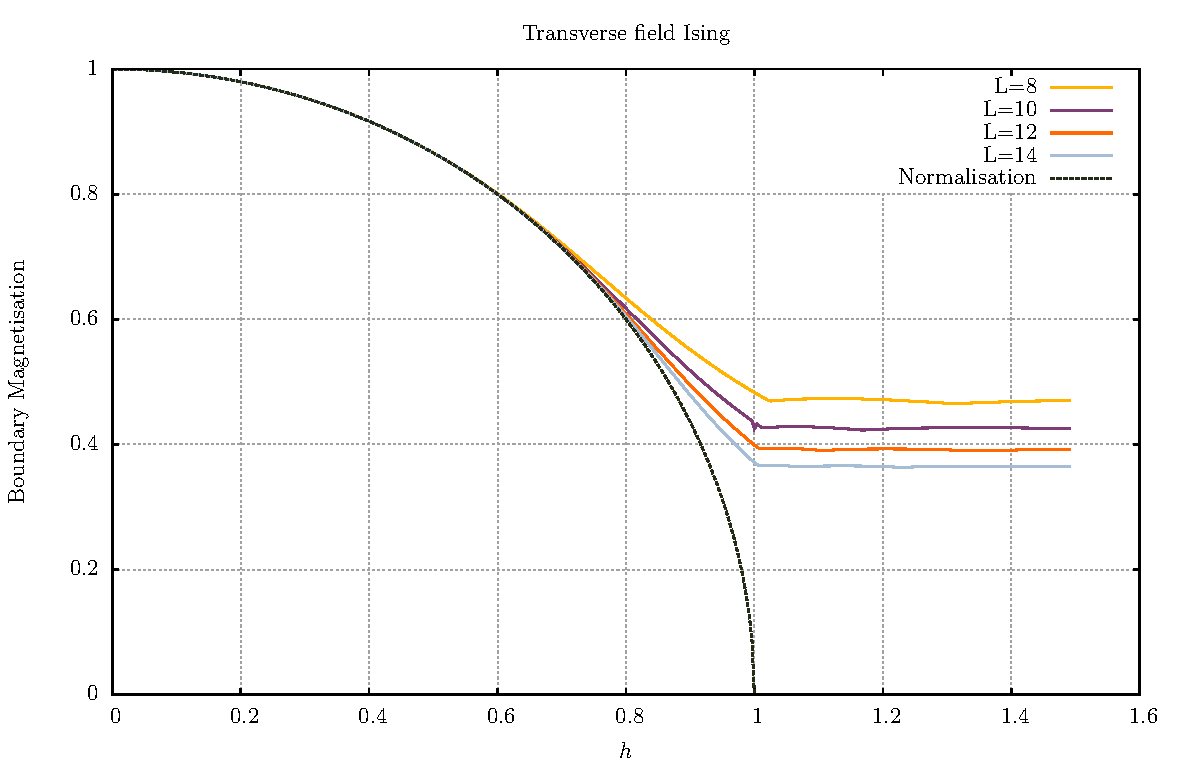
\includegraphics[width=\linewidth]{Ising_pure_magnetisation.pdf}
\caption{}
\end{subfigure}%
\begin{subfigure}{.5\textwidth}
  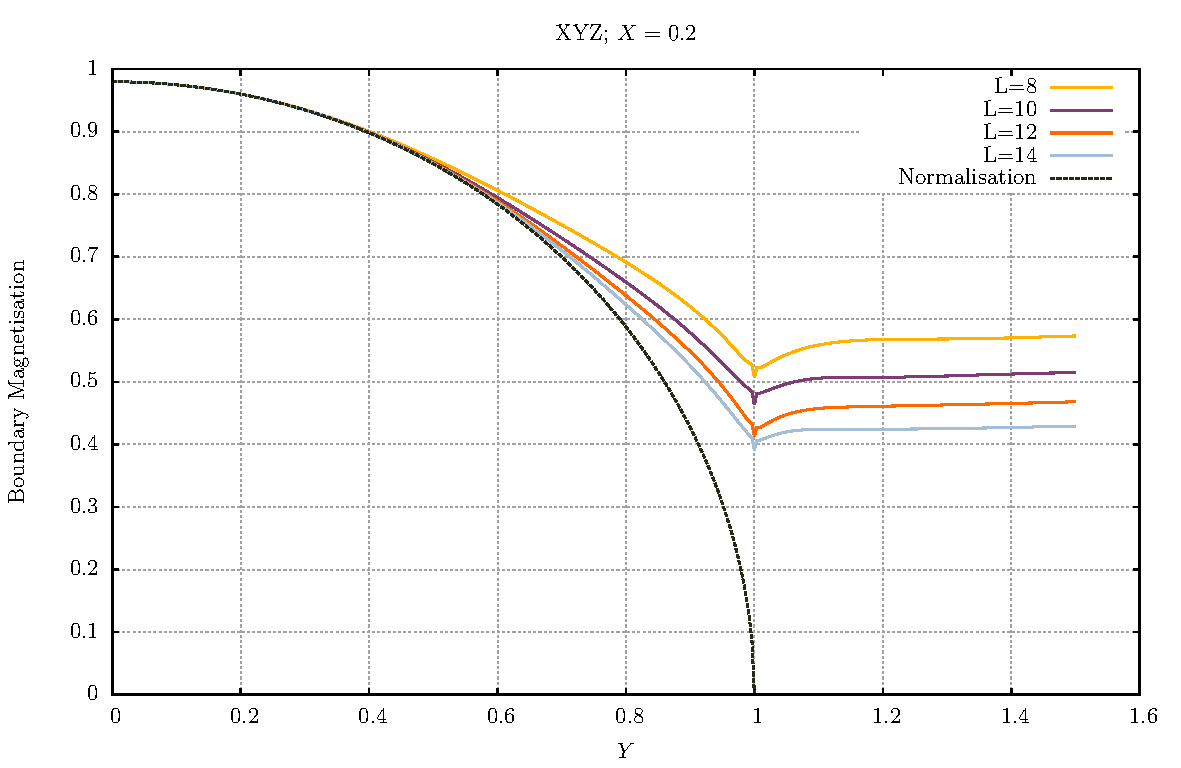
\includegraphics[width=\linewidth]{XYZ_pure_magnetisation.pdf}
\caption{}
\end{subfigure}
\caption{}
\label{fig:bmisingxyz}
\end{figure}

\subsection{Coherence times of the edge spin}
In section~\ref{sec:transisingszm} we discussed how the perturbative corrections to the SZM represented information about the initial value of the edge spin flowing into the bulk. It therefore makes sense to consider measuring the autocorrelation time of the edge spin, $\Braket{\sigma^z_1(0)\sigma^z_1(t)}$. We will see how the existence of an exact SZM implies that in the thermodynamic limit this quantity will decay to some constant, \emph{non-zero} value.

We start by introducing a resolution of the identity to decompose the expectation value into two sums over all eigenstates:
\begin{align}
\Braket{\sigma^z_1(0)\sigma^z_1(t)} &= \frac{1}{N}\sum_j \sum_k \Braket{s_j |\sigma^z_1(0)| s_k}\Braket{s_k|e^{-i H t}\sigma^z_1(0)e^{i H t}|s_j} \\
&= \frac{1}{N}\sum_j \sum_k{|\Braket{s_j |\sigma^z_1(0)| s_k}|}^2 e^{i\left(E_j-E_k\right)t},
\end{align}
where we have used the fact that the $\ket{s_j}$ are eigenstates energy $E_j$ and we have set $\hbar =1$. We see that for this quantity to remain finite there must be a macroscopic number of states with finite overlap which are close in energy, so that they remain in phase. This is of course exactly what is provided by the pairing due to a SZM. Indeed, if we assume that the other contributions dephase in the long-time limit, as in general they should, we may calculate that:
\begin{align}
 \lim_{t\to\infty}\Braket{\sigma^z_1(0)\sigma^z_1(t)} &=  \frac{1}{N}\sum_j |\Braket{s_j^\prime |\sigma^z_1(0)| s_j}|^2 \\
&= \mathcal{N}^2,
 \label{eq:decaytonorm}
\end{align}
where we have used equations~\eqref{eq:isingbm} and~\eqref{eq:xyzbm} in the last step for Ising and XYZ respectively.

Thus in the thermodynamic limit we expect $\Braket{\sigma^z_1(0)\sigma^z_1(t)}$ to decay to a constant related to the normalisation of the SZM. At finite size the SZM only commutes with the Hamiltonian up to exponentially-small terms, so eventually even the paired terms will dephase. Thus at finite size we expect to see two different time scales: a fast decay to a plateau at $\mathcal{N}^2$ due to the unpaired terms dephasing, followed by a slow decay to zero with a decay time which grows exponentially in system size due to the paired terms dephasing. We may calculate this for small system sizes using exact diagonalisation, as is shown in Figure~\cite{XYZ_decay} for XYZ.

\begin{figure} [htbp]
\centering
 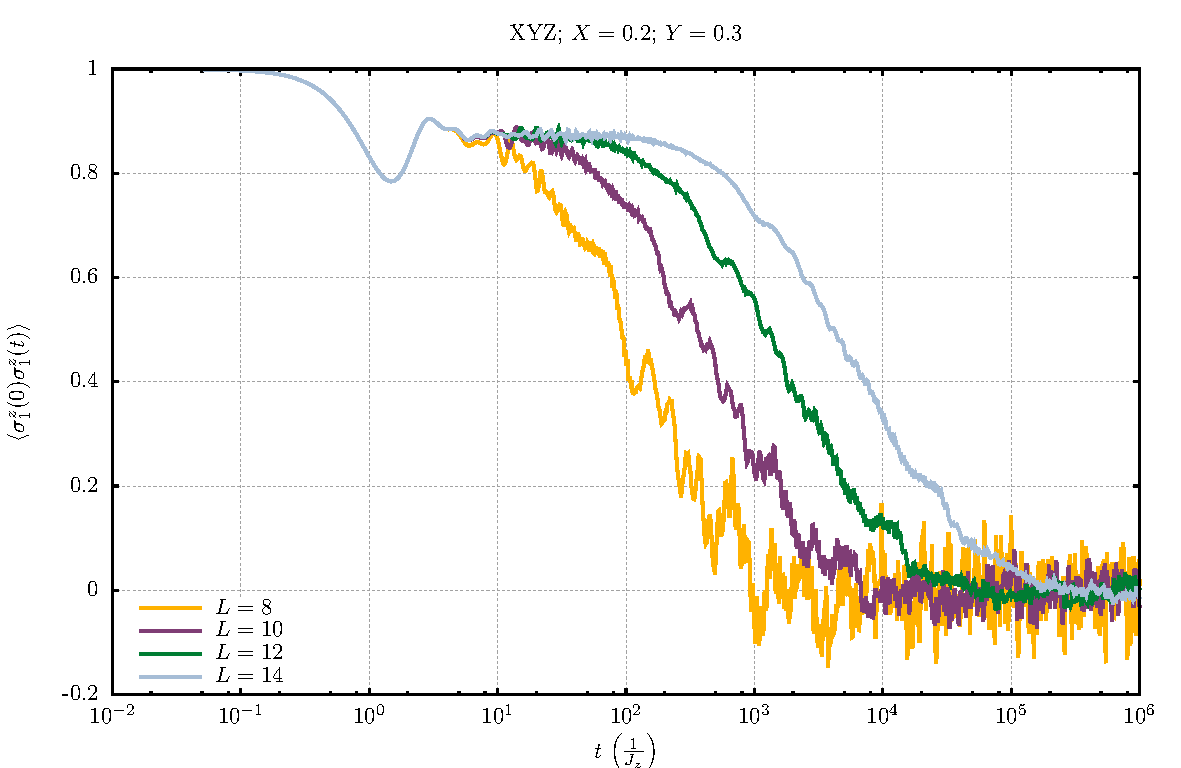
\includegraphics[width=\linewidth]{XYZ_log_decay.pdf}
\caption{}
\label{fig:XYZ_decay}
\end{figure}


We note that as an extremely non-generic case the above finite-size arguments do not apply to the pure transverse-field Ising model. As this is a model of free-fermions, in finite size it is possible to recast the SZM as a `shift' operator obeying $[H, \Psi] = \epsilon \Psi$~\cite{freefermions}. Hence all the paired states differ by exactly the same energy $\epsilon$, and so remain in phase even at finite size. Instead of decaying to zero $\Braket{\sigma^z_1(0)\sigma^z_1(t)}$ instead undergoes sinusoidal oscillations whose period is exponentially long in the system size, as shown in Figure~\ref{fig:isingdecay}.

\begin{figure} [htbp]
\centering
 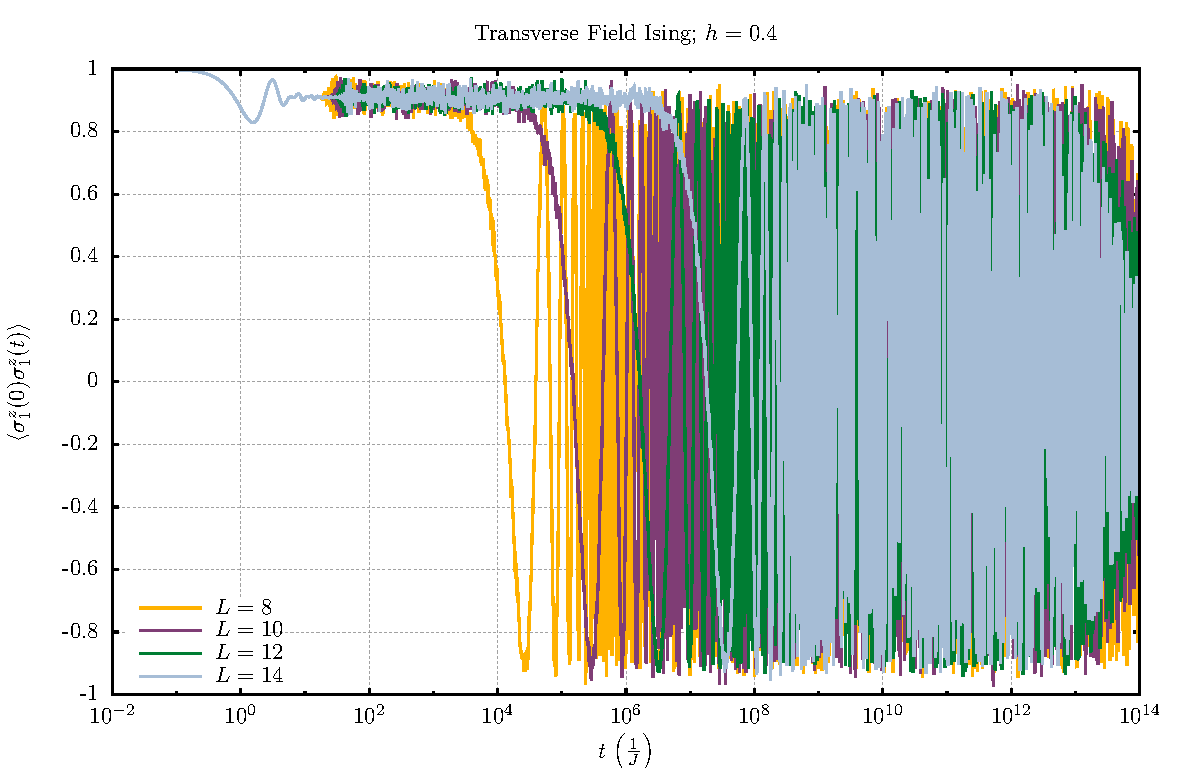
\includegraphics[width=\linewidth]{Ising_log_decay.pdf}
\caption{}
\label{fig:isingdecay}
\end{figure}

\subsection{Paired Energy Difference Variance}
\label{sec:pedv}
The oscillations observed in finite-size Ising illustrate clearly the idea that it is not the energy differences of paired states that cause a decay to zero in $\Braket{\sigma^z_1(0)\sigma^z_1(t)}$ per se, but rather their \emph{variance}, as it is this variance which drives dephasing. 

This suggests the following useful measure for the existence of the SZM and its effect on the coherence time of the edge spin, which we call the paired energy difference variance (PEDV): 
\begin{enumerate}
\item Take an eigenstate in the even sector $\ket{s_j}$. Find its paired eigenstate $\ket{s_j^\prime}$ in the odd sector by maximising the matrix element $\Braket{s_j^\prime|\sigma_z|s_j}$.
\item Calculate the difference between the energy of the two paired eigenstates $\Delta_j = E_j^\prime -E_j$.
\item Then the PEDV is given by the variance of all the energy differences: $\text{PEDV} = \text{Var}(\{\Delta_j\})$. 
\end{enumerate}
As well as indicating how consistently the SZM pairs the energy spectrum -- though, importantly, not necessarily how well the spectrum is paired without reference to the SZM -- the PEDV, or rather, its inverse, should give us an estimate of the timescale on which the decay from the plateau at $\mathcal{N}^2$ occurs.

The PEDV is plotted for XYZ when $X = 0.2$ and $Y$ is varied in Figure~\ref{fig:xyzpedv} for different system sizes. For $Y>1$, where the SZM no longer exists we see that the PEDV is large and converges in system size. For $Y<1$ the PEDV decreases as a power law in $Y$, with the power proportional to the system size $L$: that is, we have exponential corrections in $L$. Thus extrapolating to the thermodynamic limit we would expect the PEDV to become a step function from zero at $Y=1$, implying no decay in the thermodynamic limit, as we have already established we should expect.




\subsection{Physical consequences of pseudo-SZMs}
\subsection{Boundary Magnetisation}
We now turn our attention to the observable consequences in finite size of the existence of pseudo-SZMs, as described in section~\ref{sec:pseudoszm}. We first consider the boundary magnetisation, or pairing induced by the edge spin, as we described in section~\ref{sec:isingbm}. We showed in that section that as long as $\sigma^z_1$ does not reappear by itself in the perturbative expansion of the (pseudo-)SZM, then at infinite temperature the boundary magnetisation is equal to the normalisation of the SZM.

Recall that there were two ways in which the SZM could fail: firstly, an explosion of terms due to integrability-breaking causing the SZM to become unnormalisable; and secondly, poles appearing in the SZM expansion. In the former case, at any finite size we may \emph{always} choose values of the couplings small enough such that the normalisation, and thus the boundary magnetisation, is close to one. Conversely, if we keep the value of the couplings fixed and increase the system size, the divergence will ultimately force the normalisation to vanish, so that there can be no pairing in the thermodynamic limit.

This is the behaviour we observe in Figure~\ref{fig:bmgamma2}, which shows the boundary magnetisation calculated using exact diagonalisation for the Ising-like Hamiltonian given in~\eqref{eq:hamiltonian} with $J_2 = 0$. For small $\Gamma$ and $\Gamma_2$ we see that the pairing is large, but that there is a step-function transition (albeit smooth because we are at finite size) in $\Gamma_2$ to no pairing. The value of $\Gamma_2$ at which this transition occurs decreases with system size, and in the thermodynamic limit we would expect it to converge to $\Gamma_2 = 0$, which is consistent with our knowledge that an exact SZM does exist in pure transverse-field Ising. 

\begin{figure} [htbp]
\centering
 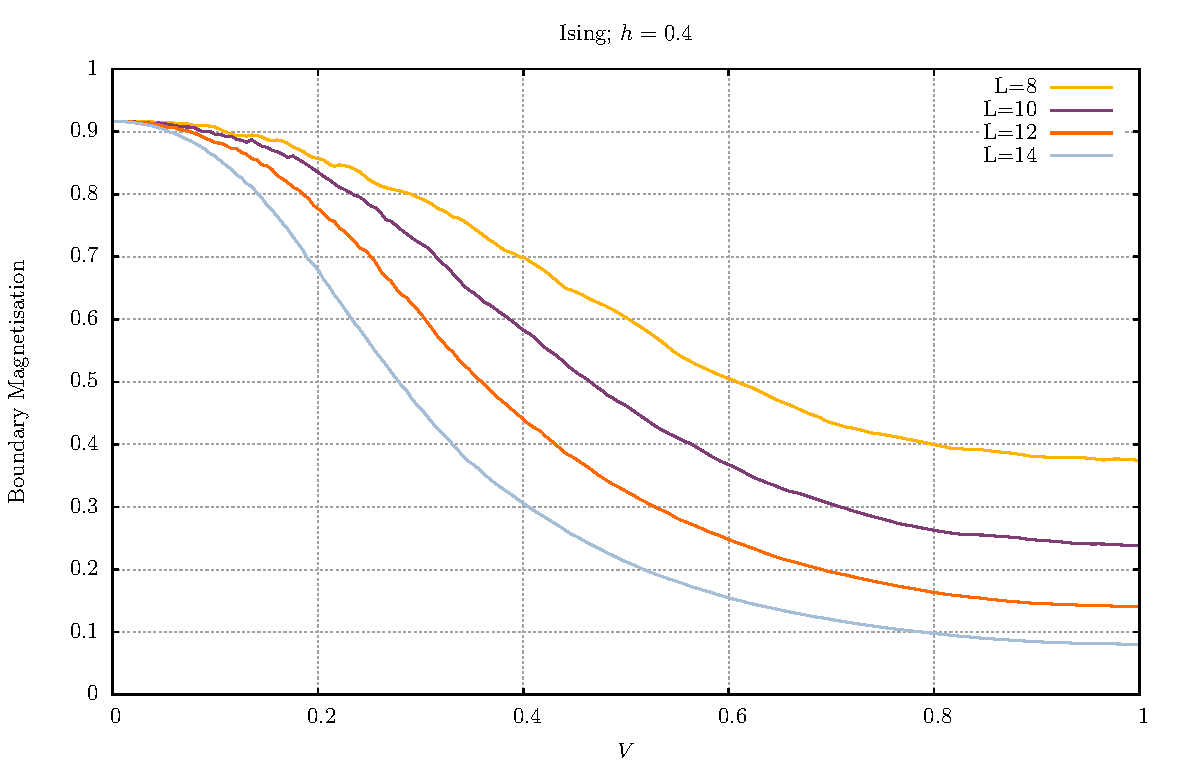
\includegraphics[width=\linewidth]{V_mag.pdf}
\caption{}
\label{fig:bmgamma2}
\end{figure}


More interestingly, we may set $\Gamma_2 = 0$ and turn on the next-nearest-neighbour coupling $J_2$. In this case poles appear in the SZM which we expect to become dense in $J_2$ and ultimately kill the SZM. These poles should appear in the boundary magnetisation, and indeed in Figure~\ref{fig:bmj2} we may clearly see the poles at $J_2 =  J$ and $J/2$. Notice that at this small value of $\Gamma$ the pairing far from the poles is almost perfect, and that the decrease in pairing even for the second order pole with system size is very slow. The graph is also symmetric about $J_2 = 0$, indicating that this structure is independent of the different ground state physics that occurs when one of the couplings is antiferromagnetic.

\begin{figure} [htbp]
\centering
 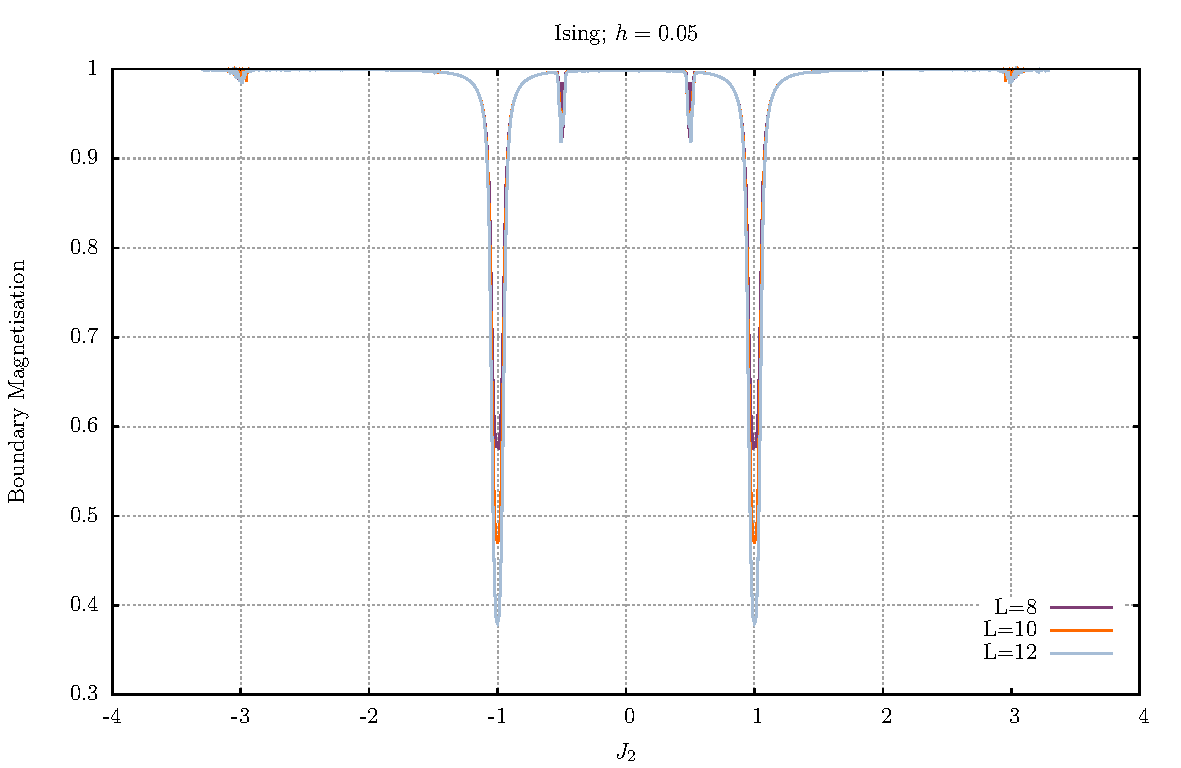
\includegraphics[width=\linewidth]{J2_mag.pdf}
\caption{}
\label{fig:bmj2}
\end{figure}

It is important to stress that normally this pairing decays as we go into the bulk if we use $\sigma^z_j$ to pair states instead of specifically the edge spin, so that this really is a special property of the edge. On the other hand the pairing in the energy spectrum need not vanish with the edge-spin pairing, as there could easily be another, not edge-localised (or even local) operator which takes one degenerate state to another. For example, at the pole at $J_2 = J$ it turns out that although the pairing due to $\sigma^z_1$ dies, the pairing due to $\sigma^z_2$ is large. Indeed, if one performs a SZM starting with $\sigma^z_2$ one finds that although it is has more terms and is in general a worse SZM than $\sigma^z_1$ it lacks the pole at $J_2 = J$. This is easy to understand by referring back to Figure~\ref{fig:domainwallfirstorder} and noting that there is no domain-wall conversion process which converts a $J$ domain wall into a $J_2$ one while flipping $\sigma^z_2$ for zero energy change. 

\subsection{Paired Energy Difference Variance}
 As the pairing only decays slowly with system size at higher order poles, it is not the best probe of the pole structure of the SZM. Furthermore, if we are interested in the coherence time of the edge spin as before, we would like to investigate how the SZM pairs the energy spectrum. This motivates the calculation of the PEDV we introduced above in section~\ref{sec:pedv}, which we plot in Figure~\ref{fig:pedvj2}.

\begin{figure} [htbp]
\centering
 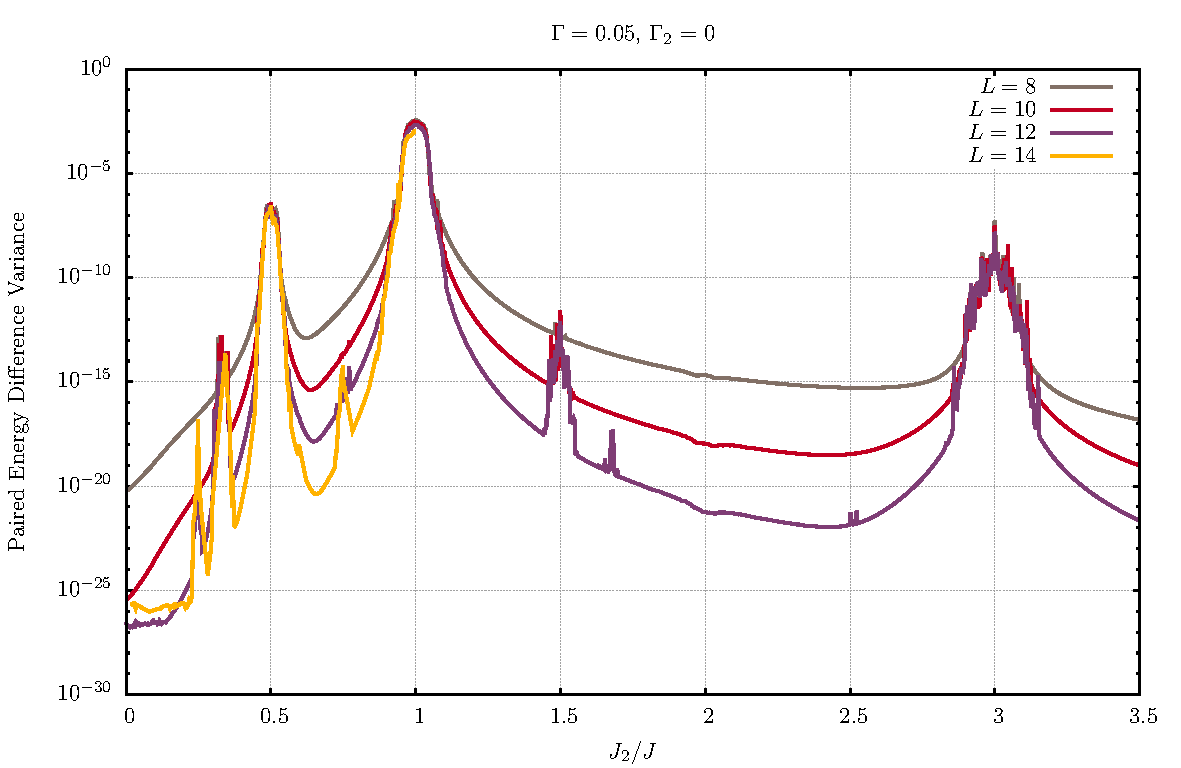
\includegraphics[width=\linewidth]{poles_lowf.pdf}
\caption{}
\label{fig:pedvj2}
\end{figure}


The pole structure is immediately apparent; not only are the first and second order poles visible but so are the third order poles at $J = J/3$, $3J/2$ and at the larger system sizes even fourth order poles at $J_2 = J/4$ and $3 J/4$. We calculated the perturbative SZM expansion up to third order and these poles coincide precisely with those in the PEDV (albeit there is another third order pole at $J_2 = 5 J$ not visible on this axis), and the fourth order poles follow the same general pattern we would expect. Notice the log scale on the y axis: this structure in the PEDV thus traverses almost 30 orders of magnitude!

Away from the poles the PEDV exponentially decreases with system size. This is exactly the same as for the XYZ case in Figure~\ref{fig:xyzpedv}, and as already explained may be understood as the finite-size behaviour of an exact SZM. Of course, we do not expect this exponential decrease to survive to the thermodynamic limit, as eventually \emph{all} points will lie on a pole.

On the other hand, close to the poles it appears the PEDV saturates with $L$. In fact a closer look at the first order pole at $J_2 = J$ reveals the log scale is hiding a not-exponential but still substantial decrease in the peak of the pole with $L$. Nevertheless, at the full width of the pole (see below) where the cross-over to finite-size behaviour occurs, the PEDV curves for different $L$ intersect. This suggests that the peak value must ultimately saturate with $L$, and indeed this is observed for much larger system sizes, see Figure~\ref{fig:saturatepeak}. This saturation with $L$ implies that the decay time of the autocorrelation of the edge spin $\Braket{\sigma^z_1(0)\sigma^z_1(t)}$ will also saturate with $L$ at the poles, rather than increasing exponentially.

\begin{figure} [htbp]
\centering
g 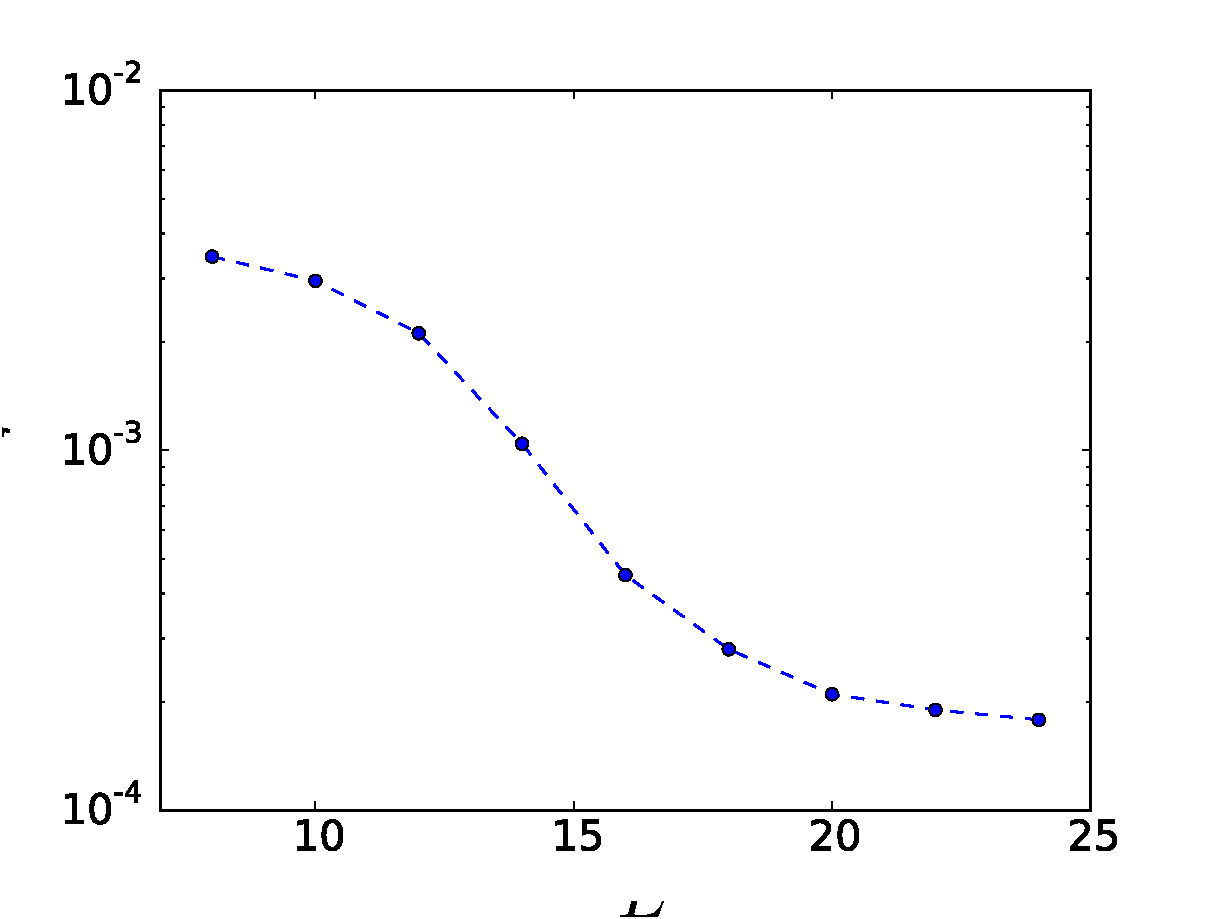
\includegraphics[width=\linewidth]{kemp_height.pdf}
\caption{}
\label{fig:saturatepeak}
\end{figure}

Before we discuss the behaviour of the pole structure as we vary $\Gamma$, we note that as plotted the PEDV has been calculated for $\Gamma$ and $J_2$ on two very different scales. A model which similarly had two very different scales has already been considered in the context of many-body localisation by Papic~\textit{et al.} in~\cite{minibands}. They considered a Hamiltonian with heavy and light fermions hopping on a lattice, and found that the numerics on small system sizes led to spurious signs of localisation due to existence of `minibands': gaps in the density of states which opened up because of the large difference between the two mass scales. We also observe minibands in our numerics. These are most promient when $J_2$ is a rational (or even more so, integer) multiple of $J$ as this reduces the number of minibands possible. Nevertheless, we are confident that the physics we are interested in is entirely independent of these minibands. This is because:
\begin{enumerate}
\item As noted, minibands occur most prominetly when $J_2$ is a rational multiple of $J$. This often, but \emph{not} always, where we observe poles in the PEDV. And poles in the PEDV are points of \emph{least} localisation, not greater, as it is here the edge-localised zero mode dies.
\item If we replace the $\Gamma$ term by the $\Gamma_2$ term, and repeat the calculation, we find the poles change in position and relative magnitude exactly as predicted by the SZM expansion, but not by any miniband structure, which should remain the same regardless of which disordering term we use as long as they are of similar magnitude.
\end{enumerate}

How then does the height and width of the poles change as we vary $\Gamma$? Both of these quantities may be easily estimated by recalling the domain-wall flavour conversion argument we used to explain the existence of the poles. The rate at which we expect these processes to occur, which should be proportional to the peak PEDV, must itself be proportional to the square of matrix element connecting the before and after states in perturbation theory. So for example, in order to convert at $J$ domain wall to $J_2$ for zero energy at $J_2 = J$, we must flip one spin; we therefore expect the height of the first peak to be proportional to $\Gamma^2$. Clearly in general then the height should be proportional to $\Gamma^{2 (\text{Order of pole})}$. There is strong evidence for this numerically for the first and second order poles; see figure~\ref{fig:poleheight}.

\begin{figure} [htbp]
\centering
\begin{subfigure}{.33\textwidth}
 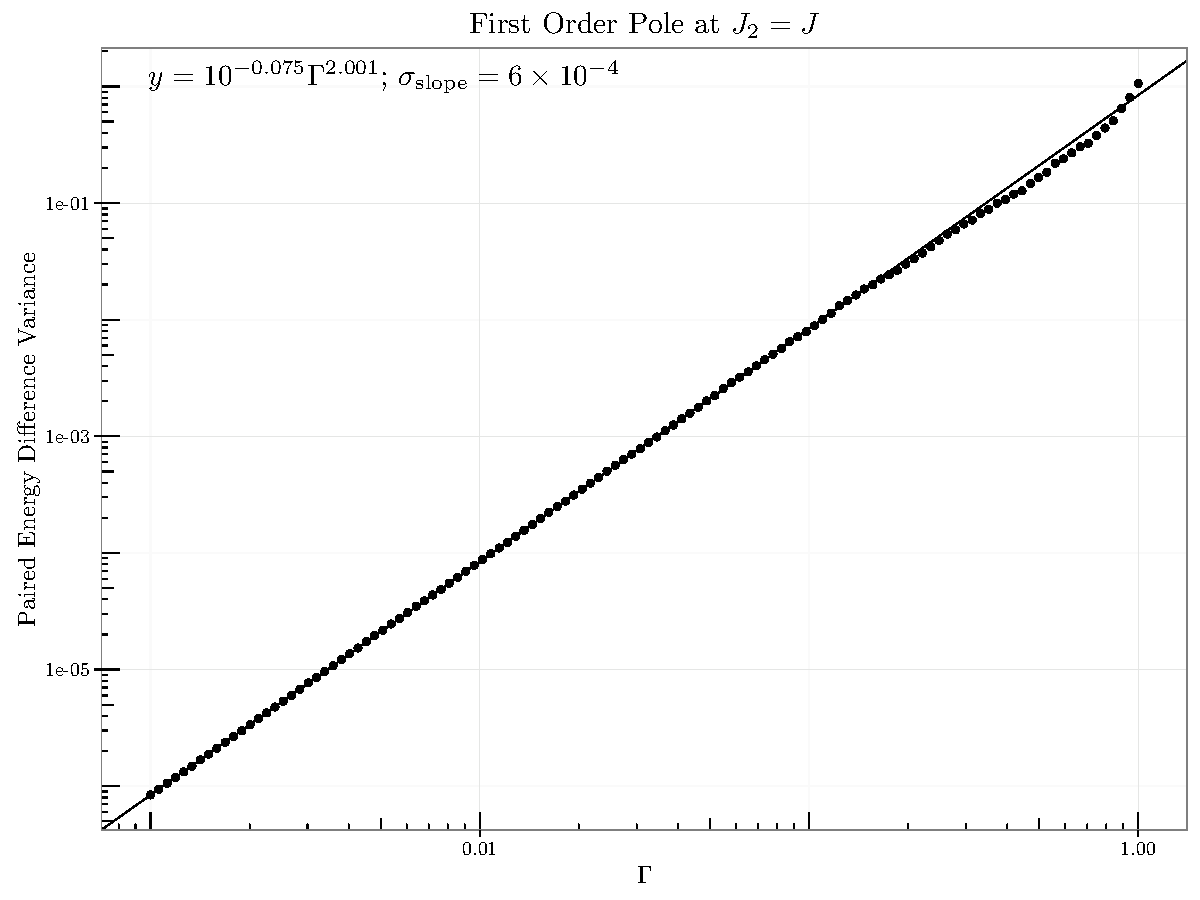
\includegraphics[width=\linewidth]{pole1_gamma_dep.pdf}
\caption{}
\end{subfigure}%
\begin{subfigure}{.33\textwidth}
  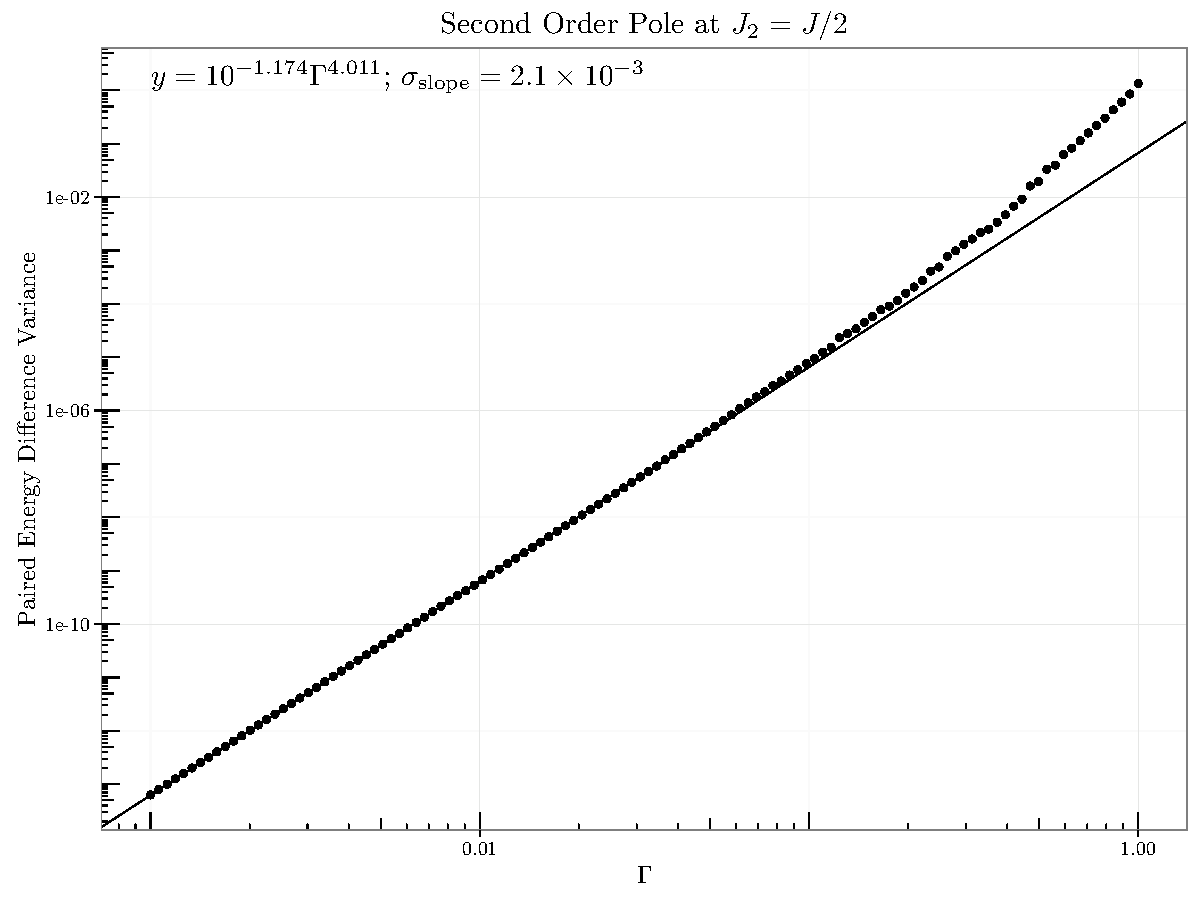
\includegraphics[width=\linewidth]{pole5_gamma_dep.pdf}
\caption{}
\end{subfigure}
\begin{subfigure}{.33\textwidth}
  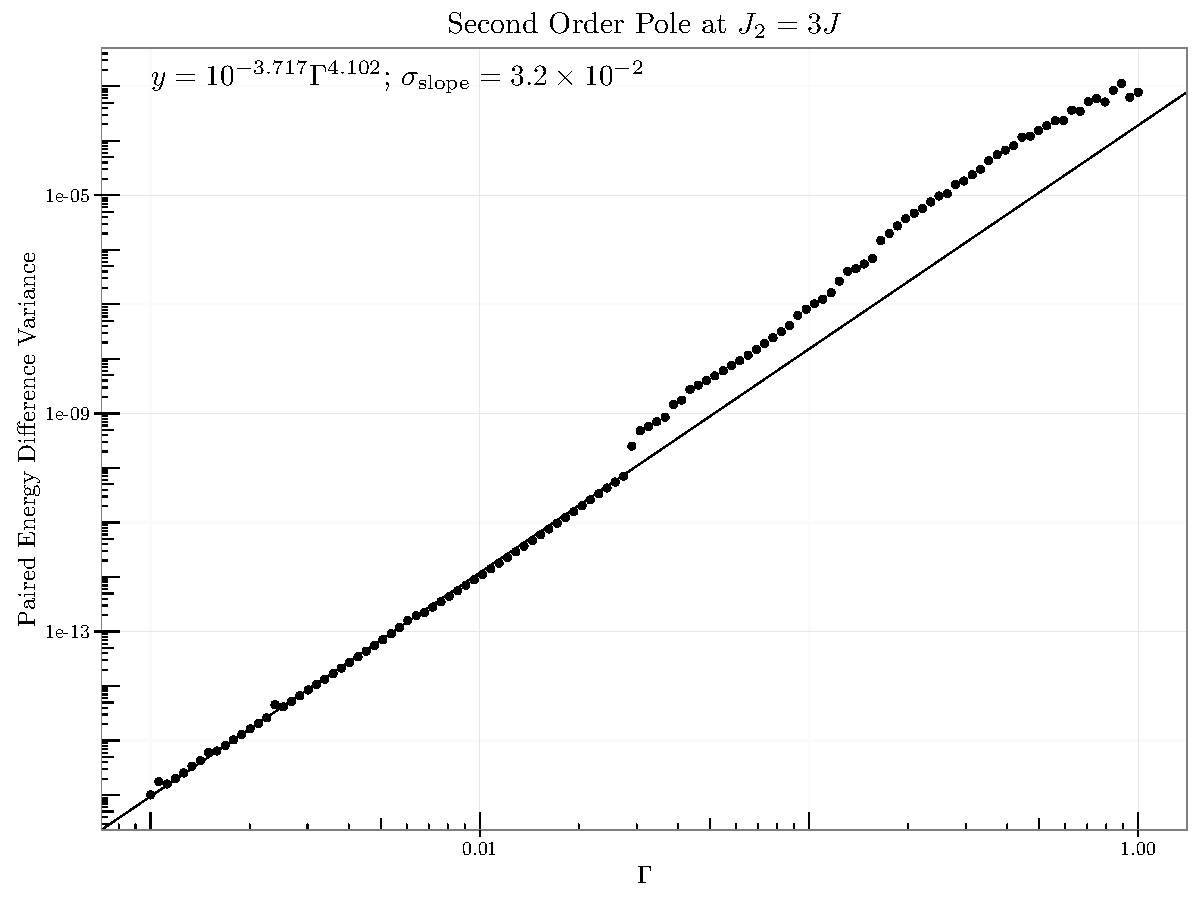
\includegraphics[width=\linewidth]{pole30_gamma_dep.pdf}
\caption{}
\end{subfigure}
\caption{}
\label{fig:poleheight}
\end{figure}

The width of the poles may be similarly estimated using such simple arguments. Notice that for finite $\Gamma$ domain walls do not last forever but instead have a finite lifetime and therefore an energy uncertainty $\approx \Gamma$. When we plot the PEDV against $J_2$, we are implicitly testing domain wall conversion processes where we know the energy of the $J_2$ domain walls we are sending in, but are affected by the energy uncertainty of the produced $J$ domain walls. So for example close to the $J_2 = 3 J$ pole, we are sending one $J_2$ domain wall in to be converted to three $J$ domain walls each with associated energy uncertainty $\Gamma$: thus we would expect the half-width of the pole in $J_2$ to be $3 \Gamma$. Conversely, at $J_2 = J/2$ we convert two $J_2$ domain walls to only one $J$ domain wall, so the half-width is reduced to $\Gamma/2$. In general we would expect the half-width to be $\frac{J_2}{J} \Gamma$, and this is supported numerically, see Figure~\ref{fig:width}.

\begin{figure} [htbp]
\centering
 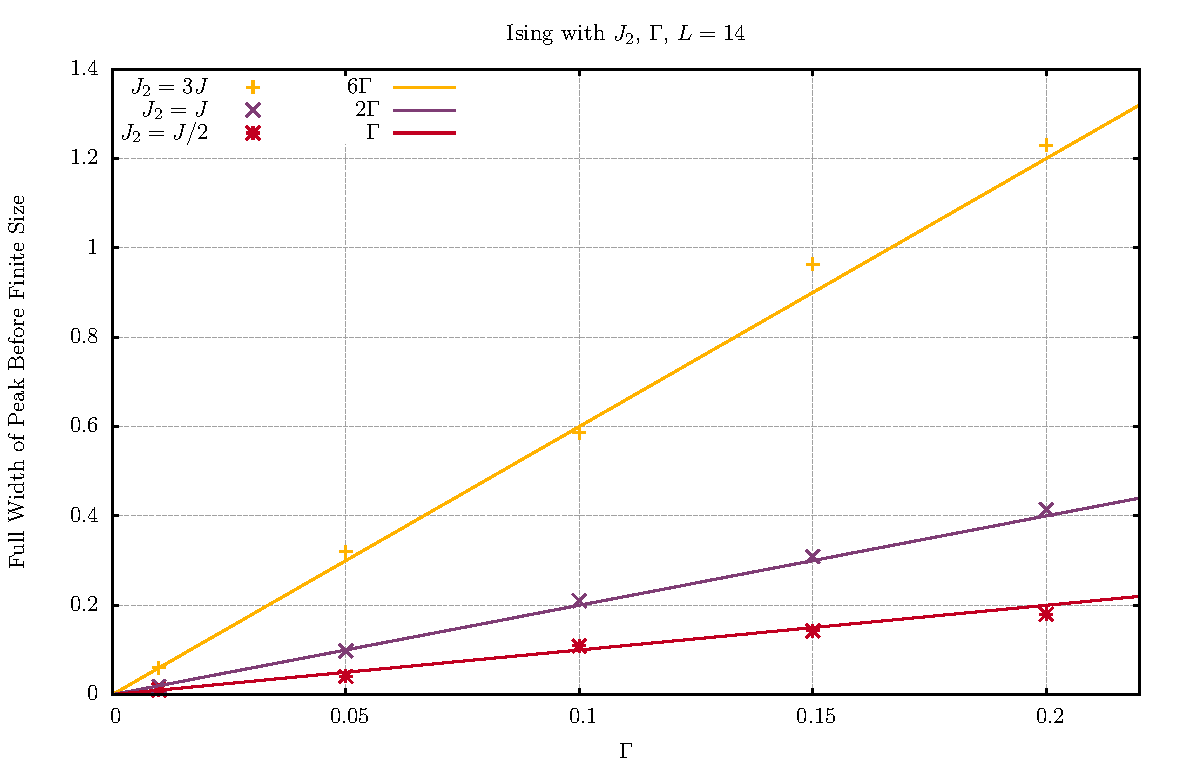
\includegraphics[width=\linewidth]{width_of_poles.pdf}
\caption{}
\label{fig:width}
\end{figure}

Both the estimates for the height and width of the PEDV poles break down if we take $\Gamma$ to be too large. At large values of $\Gamma$ the poles begin to merge, and we must also concern ourselves with higher order processes from the same pole: that is, domain wall conversion processes which flip more spins than necessary to produce the same effect as the lowest order term. Nevertheless, for large $\Gamma$ but small $J_2$ one may still find a heuristic formula for the decay time of $\Braket{\sigma^z_1(0)\sigma^z_1(t)}$; we discuss this in depth in our accompanying paper~\cite{flashypaper}.

\subsection{Coherence times of the edge spin}
From the PEDV, we should already know what we should observe on calculating the autocorrelation time of the edge spin $\Braket{\sigma^z_1(0)\sigma^z_1(t)}$ for models with pseudo-SZMs. As for an exact SZM we should expect a fast decay to a plateau whose height is related to the normalisation of the SZM, and whose duration should increase exponentially with system size. However, unlike exact SZMs, as pseudo-SZMs are ultimately unnormalisable, as we increase system size the amplitude of this plateau will decrease, until in the thermodynamic limit there will simply be a fast decay to zero.

Furthermore, if there are poles in the SZM then close to a pole the decay time should saturate in system size, rather than exponentially increasing, due to the corresponding saturation in the PEDV. This should also lead to decay times which are highly non-monotonic in $J_2$, which may be surprising if $J_2$ is viewed simply as an integrability-breaking parameter. All this behaviour appears numerically as expected, and the non-monotonicity for example is clearly visible in Figure~\ref{fig:j2decay}.

\begin{figure} [htbp]
\centering
 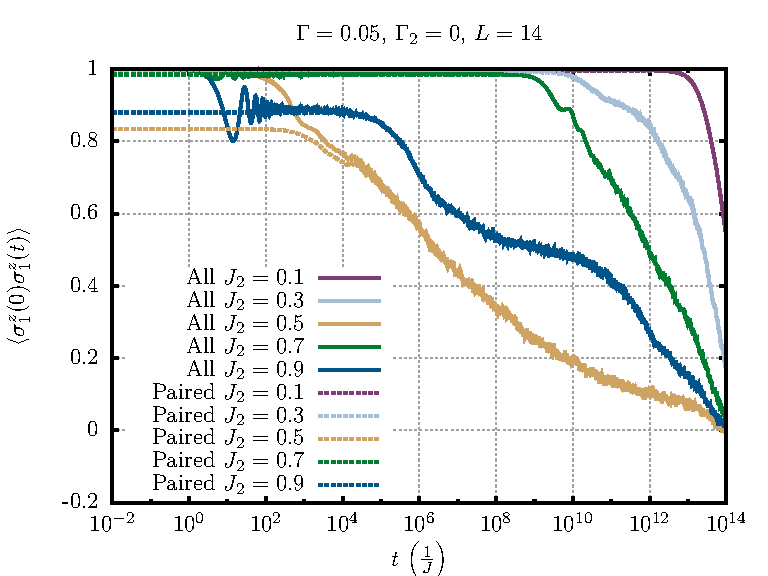
\includegraphics[width=\linewidth]{J2_decay.pdf}
\caption{}
\label{fig:j2decay}
\end{figure}

Figure~\ref{fig:j2decay} also contains a final check on our arguments, which described the plateau and subsequent slow decay entirely in terms of the paired states, assuming that all the other contributions quickly dephased to zero. The dotted lines show the same two-point function calculated using only the paired states. We see that after the initial fast dephasing the dotted and solid lines are indeed in very good agreement.

\section{Conclusion}







 









\end{document}
% LocalWords: Majorana Ising SZM Pauli
